\documentclass[12pt]{article}
\usepackage[english]{babel}
\usepackage[utf8x]{inputenc}
\usepackage{amsmath}
\usepackage{tikz}
\usetikzlibrary{arrows,automata}
\begin{document}

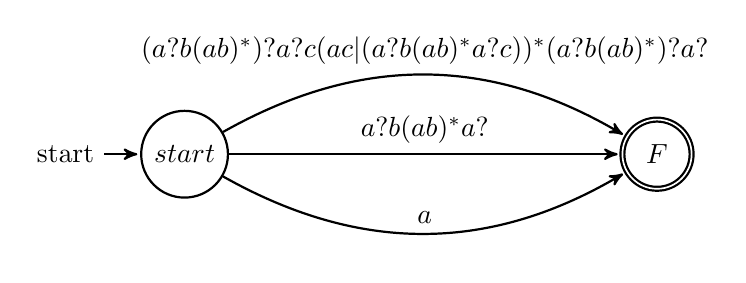
\begin{tikzpicture}[->,>=stealth',shorten >=1pt,auto,node distance=6cm,
    thick,base node/.style={circle,draw,minimum size=8pt}, real node/.style={double,circle,draw,minimum size=17pt}]

  \node[state,initial] (start) {$start$};
 
  \node[state,accepting] (F) [right of=start] {$F$};
  
  \path 
        (start) edge [bend right] node {$a$} (F)
        (start) edge node {$a?b(ab)^{*}a?$} (F)
        (start) edge  [bend left] node {$(a?b(ab)^{*})?a?c(ac|(a?b(ab)^{*}a?c))^{*}(a?b(ab)^{*})?a?$}(F)
;
\end{tikzpicture}
\end{document}